\chapter{OTA Basics}


\begin{figure}[H]
\centering
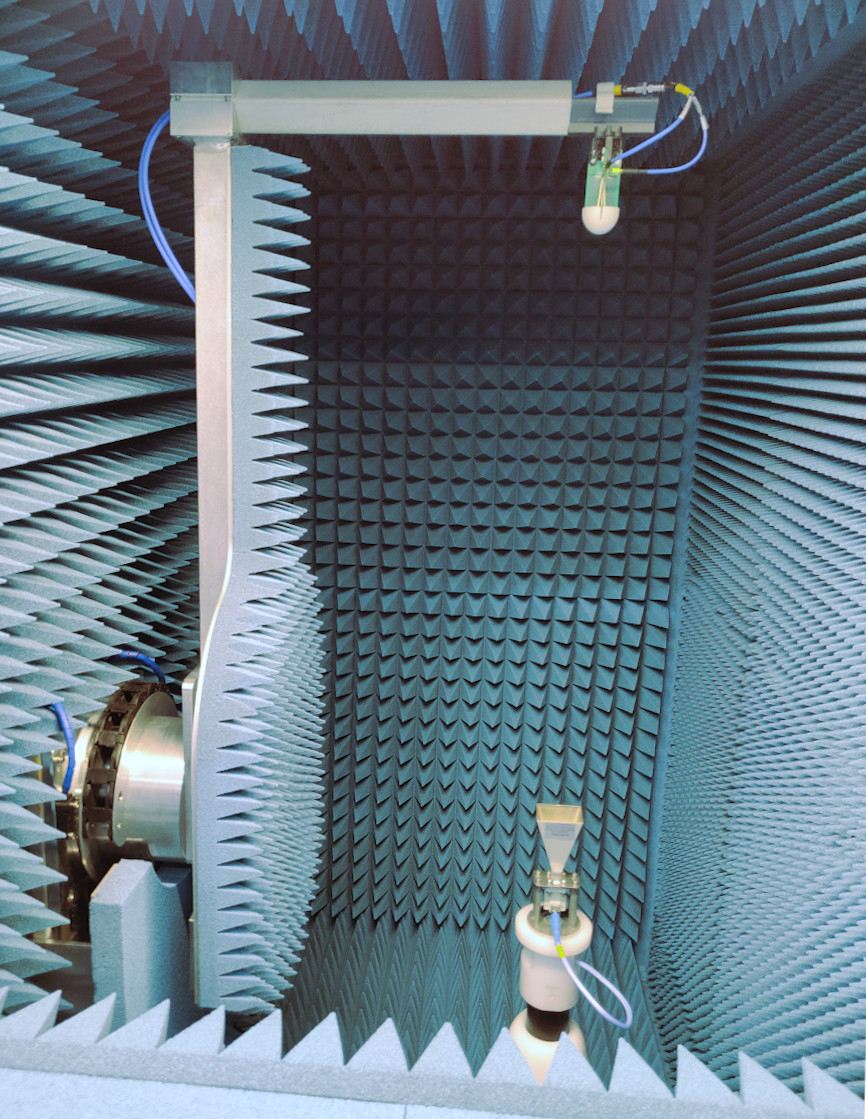
\includegraphics[width=0.4\textwidth]{ats1000.jpg}
\caption{Calibration of an ATS1000 from R\&{}S}
\label{fig:ats}
\end{figure}

This chapter gives an overview over the difficulties and solutions of \ac{OTA}-measurements. There are four main architectures for \ac{OTA}-measurement.

\begin{enumerate}
\item \textbf{\ac{RVC}}: The \ac{RVC} is fully screened inside, which makes it a resonator. Because the \ac{EM} field inside is very inhomogeneous (standing waves) there are several so called stirrers to generate random \ac{EM} modes. With a \ac{RVC} \ac{EM} emission in arbitrary direction can be measured using a fixed antenna.
\item \textbf{\ac{AC}}:
\item \textbf{\ac{CATR}}:
\item \textbf{\ac{OATS}}: \ac{OATS}
\end{enumerate}

\todo{AC weil positioner einfacher und spiegel teuer, stirrer}

\section{Setting up a OTA-measurement}

It is 
\cite{ctiaat}
\section{Link Budget}

\section{Quiet Zone}

\section{Detector Settings}

\begin{figure}[h]
\centering
\def\svgwidth{0.7\textwidth}
\input{Bilder/detectorSetting.pdf_tex}
\caption{Comparison of Detector Settings \cite{funsspec}}
\label{fig:detset}
\end{figure}

With the detector a certain sample in a given interval is chosen, compare figure \ref{fig:detset}. There are six main settings for the detector: \cite{funsspec}
\begin{itemize}
\item The \textcolor[RGB]{237,28,36}{Max Peak-detector} takes the maximum value in the give interval.
\item The \textcolor[RGB]{0,166,88}{Min Peak-detector} takes the minimum value in the give interval.
\item The \textcolor[RGB]{0,94,138}{Auto Peak-detector} displays the interval from Min- to Max-Peak.
\item The \textcolor[RGB]{0,173,239}{Sample-detector} takes the first value in the give interval.
\item The \textcolor[RGB]{246,135,18}{RMS-detector} computes the \ac{RMS} of the signal to display.
\item The \textcolor[RGB]{114,100,184}{AV-detector} computes the average of the signal to display.
\end{itemize}

Choosing the \glqq right\grqq{ } detector setting is dependent of the expected signal. If a stochastic signal (noise) is to be found, the \ac{RMS}-detector is always the right choice. If it is harmonic, the Max Peak-detector is right. There are tow major problems:

\begin{enumerate}
\item By using the Peak-detector for measuring stochastic signals the minimum error is $\SI{2.5}{\decibel}$ when the frequency intervals are short (a lot of display points).
\item If the \ac{RMS}- or AV-detector is used harmonic signals are underrated dependent from the interval length caused by the averaging.
\end{enumerate} 

For a coarse pre scan a Peak-detector is normally used and if something is found a fine scan is carried out with \ac{RMS}-detector at the interesting frequencies.


